\documentclass{standalone}
\usepackage{tikz}
\usepackage{amsmath}

\begin{document}

\tikzset{every picture/.style={line width=0.75pt}} %set default line width to 0.75pt

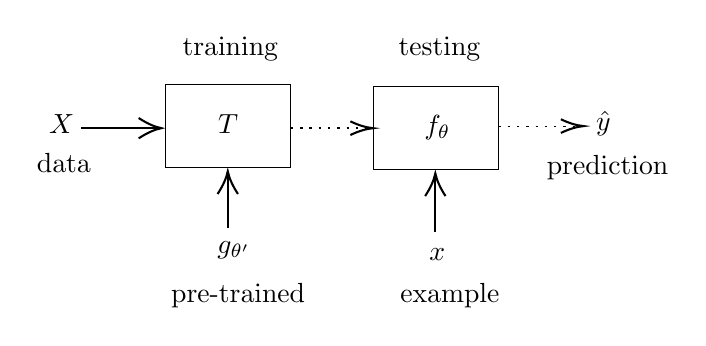
\begin{tikzpicture}[x=0.75pt,y=0.75pt,yscale=-1,xscale=1]
% uncomment if require:
% \path (0,300); %set diagram left start at 0, and has height of 300

%Straight Lines [id:da47504456322753597]
\draw [line width=0.75]    (140.42,91.23) -- (178.42,91.23) ;
\draw [shift={(179,91.23)}, rotate = 180] [color={rgb, 255:red, 0; green, 0; blue, 0 }  ][line width=0.75]    (10.93,-4.9) .. controls (6.95,-2.3) and (3.31,-0.67) .. (0,0) .. controls (3.31,0.67) and (6.95,2.3) .. (10.93,4.9)   ;

%Shape: Rectangle [id:dp7482618074258622]
\draw   (181,70) -- (241.42,70) -- (241.42,110) -- (181,110) -- cycle ;
%Straight Lines [id:da18397168745182513]
\draw [line width=0.75]    (211,139.23) -- (211,112.23) ;
\draw [shift={(211,112)}, rotate = 450] [color={rgb, 255:red, 0; green, 0; blue, 0 }  ][line width=0.75]    (10.93,-4.9) .. controls (6.95,-2.3) and (3.31,-0.67) .. (0,0) .. controls (3.31,0.67) and (6.95,2.3) .. (10.93,4.9)   ;

%Straight Lines [id:da1497519588402466]
\draw [line width=0.75]  [dash pattern={on 0.84pt off 2.51pt}]  (241.42,91.23) -- (280.42,91.23) ;
\draw [shift={(281,91.23)}, rotate = 180] [color={rgb, 255:red, 0; green, 0; blue, 0 }  ][line width=0.75]    (10.93,-3.29) .. controls (6.95,-1.4) and (3.31,-0.3) .. (0,0) .. controls (3.31,0.3) and (6.95,1.4) .. (10.93,3.29)   ;

%Shape: Rectangle [id:dp8004262624933598]
\draw   (281,71) -- (341.42,71) -- (341.42,111) -- (281,111) -- cycle ;
%Straight Lines [id:da34977670625280843]
\draw [line width=0.75]    (311,141.23) -- (311,114.23) ;
\draw [shift={(311,113)}, rotate = 450] [color={rgb, 255:red, 0; green, 0; blue, 0 }  ][line width=0.75]    (10.93,-4.9) .. controls (6.95,-2.3) and (3.31,-0.67) .. (0,0) .. controls (3.31,0.67) and (6.95,2.3) .. (10.93,4.9)   ;

%Straight Lines [id:da568055817791514]
\draw  [dash pattern={on 0.84pt off 2.51pt}]  (341.42,90.23) -- (380.42,90.23) ;
\draw [shift={(382.42,90.23)}, rotate = 180] [color={rgb, 255:red, 0; green, 0; blue, 0 }  ][line width=0.75]    (10.93,-3.29) .. controls (6.95,-1.4) and (3.31,-0.3) .. (0,0) .. controls (3.31,0.3) and (6.95,1.4) .. (10.93,3.29)   ;


% Text Node
\draw (131,89) node(data)   {$X$};
% Text Node
\draw (214,150) node(pretr)   {$g_{\theta '}$};
% Text Node
\draw (312,152) node(example)   {$x$};
% Text Node
\draw (392,89) node(pred)   {$\hat{y}$};
% Text Node
\draw (312,91) node   {$f_{\theta }$};
% Text Node
\draw (216,172) node   {$\text{pre-trained}$};
% Text Node
\draw (132,108) node   {$\text{data}$};
% Text Node
\draw (318,172) node   {$\text{example}$};
% Text Node
\draw (394,110) node   {$\text{prediction}$};
% Text Node
\draw (212.21,53) node   {$\text{training}$};
% Text Node
\draw (313,53) node   {$\text{testing}$};
% Text Node
\draw (211.21,89) node   {$T$};


\end{tikzpicture}

\end{document}
